% Number 720
% GM UCM Kepler Algebra Units Vectors
% Planet orbiting Sun - circular, elliptical
% JG

% Watermark
\AddToShipoutPicture*{\BackgroundPic}

\addtocounter {ProbNum} {1}

%\begin{floatingfigure}[r]{.42\textwidth}
%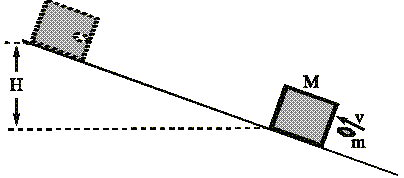
\includegraphics[scale=.6]{/Users/jgates/desktop/latex/pics/inclinebulletblock}
%\end{floatingfigure}
 
{\bf \Large{\arabic{ProbNum}}} A planet orbits the Sun twice as far from the Sun as the Earth is.  Assume that the planet's orbit and the Earth's orbit are circular.

\bigskip
Determine, in two different ways, the orbital period of this planet. You may look up any values that you need.\paragraph{}
\noindent
\vfill

\begin{floatingfigure}[r]{.26\textwidth}
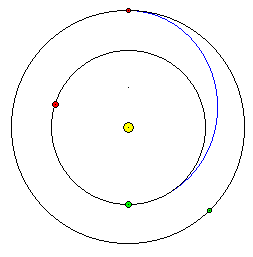
\includegraphics[scale=.6]{/Users/jgates/desktop/latex/pics/hohmann1}
\end{floatingfigure}

One way to transfer from the Earth to the new planet is to use an elliptical transfer orbit. This orbit begins at the Earth (inner planet) and ends at the new (outer) planet.  Determine the length of the semi-major axis of this orbit and how long it will take astronauts to travel from the Earth to this new planet.
\vfill
%\hfill 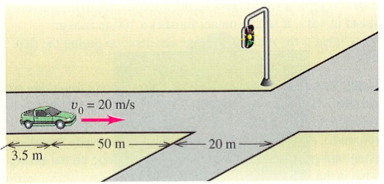
\includegraphics[scale=.85]{/Users/jgates/desktop/latex/pics/redlight.png}
\newpage